% -*- coding: utf-8; -*-
% vim: set fileencoding=utf-8 :
\documentclass[english,submission]{programming}
%% First parameter: the language is 'english'.
%% Second parameter: use 'submission' for initial submission, remove it for camera-ready (see 5.1)

\usepackage[backend=biber]{biblatex}
\addbibresource{example.bib}


%
% Packages and Commands specific to article (see 3)
%
% These ones  are used in the guide, replace with your own.
% 
%% \usepackage{multicol}
%% \usepackage{ccicons}
%% \lstdefinelanguage[programming]{TeX}[AlLaTeX]{TeX}{%
%%   deletetexcs={title,author,bibliography},%
%%   deletekeywords={tabular},
%%   morekeywords={abstract},%
%%   moretexcs={chapter},%
%%   moretexcs=[2]{title,author,subtitle,keywords,maketitle,titlerunning,authorinfo,affiliation,authorrunning,paperdetails,acks,email},
%%   moretexcs=[3]{addbibresource,printbibliography,bibliography},%
%% }%
%% \lstset{%
%%   language={[programming]TeX},%
%%   keywordstyle=\firamedium,
%%   stringstyle=\color{RosyBrown},%
%%   texcsstyle=*{\color{Purple}\mdseries},%
%%   texcsstyle=*[2]{\color{Blue1}},%
%%   texcsstyle=*[3]{\color{ForestGreen}},%
%%   commentstyle={\color{FireBrick}},%
%%   escapechar=`,}
%% \newcommand*{\CTAN}[1]{\href{http://ctan.org/tex-archive/#1}{\nolinkurl{CTAN:#1}}}
%%


%%%%%%%%%%%%%%%%%%
%% These data MUST be filled for your submission. (see 5.3)
\paperdetails{
  %% perspective options are: art, sciencetheoretical, scienceempirical, engineering.
  %% Choose exactly the one that best describes this work. (see 2.1)
  perspective=art,
  %% State one or more areas, separated by a comma. (see 2.2)
  %% Please see list of areas in http://programming-journal.org/cfp/
  %% The list is open-ended, so use other areas if yours is/are not listed.
  area={Smalltalk},
  %% You may choose the license for your paper (see 3.)
  %% License options include: cc-by (default), cc-by-nc
  % license=cc-by,
}
%%%%%%%%%%%%%%%%%%

%%%%%%%%%%%%%%%%%%
%% These data are provided by the editors. May be left out on submission.
%\paperdetails{
%  submitted=2016-08-10,
%  published=2016-10-11,
%  year=2016,
%  volume=1,
%  issue=1,
%  articlenumber=1,
%}
%%%%%%%%%%%%%%%%%%


\begin{document}

\title{The First Fifty Years of Smalltalk}
\subtitle{Smalltalk-76 as the ur-Object-Oriented Programming Model}% optional
\titlerunning{Fifty Years of Smalltalk-76} %optional, in case that the title is too long; the running title should fit into the top page column

\author[a]{James Noble}[0000-0001-9036-5692]
\authorinfo{Visiting International Chair. 
  \email{james.noble@programming.ac.nz}.}
\affiliation[a]{INRIA Lille, France}

\author{Your Name Here}[0000-0000-0000-0000]
\authorinfo{Visiting International Chair. 
  \email{your.name.jere@inria.fr}.}
\affiliation{INRIA Lille, France}


%% \author{Cristina V. Lopes}[orcid.org/0000-0003-0551-3908]
%% \authorinfo{is associate editor for the first two issues of The Art, Science,
%%   and Engineering of Programming. Contact her at \email{lopes@ics.uci.edu}.}
%% \affiliation{University of California, Irvine, USA}
%% \author[a]{Robert Hirschfeld}[https://orcid.org/0000-0002-4249-6003]
%% \authorinfo{is chair of the AOSA steering committee. The Art, Science,
%%   and Engineering of Programming is published by AOSA. Contact Robert at \email{hirschfeld@hpi.uni-potsdam.de}.}

\authorrunning{J. Noble et al.}

\keywords{Smalltalk, language, design, bytecodes, meta-model.} % please provide 1--5 keywords


%%%%%%%%%%%%%%%%%%%%%%%%%%%%%
% Please go to https://dl.acm.org/ccs/ccs.cfm and generate your Classification
% System [view CCS TeX Code] stanz and copy _all of it_ to this place.
%% From HERE
\begin{CCSXML}
<ccs2012>
   <concept>
       <concept_id>10011007.10011006.10011008.10011009.10011011</concept_id>
       <concept_desc>Software and its engineering~Object oriented languages</concept_desc>
       <concept_significance>500</concept_significance>
       </concept>
   <concept>
       <concept_id>10011007.10011006.10011008.10011024.10011029</concept_id>
       <concept_desc>Software and its engineering~Classes and objects</concept_desc>
       <concept_significance>500</concept_significance>
       </concept>
   <concept>
       <concept_id>10011007.10011006.10011041.10010943</concept_id>
       <concept_desc>Software and its engineering~Interpreters</concept_desc>
       <concept_significance>300</concept_significance>
       </concept>
   <concept>
       <concept_id>10003456.10003457.10003521.10003525</concept_id>
       <concept_desc>Social and professional topics~History of programming languages</concept_desc>
       <concept_significance>300</concept_significance>
       </concept>
 </ccs2012>
\end{CCSXML}
\ccsdesc[500]{Software and its engineering~Object oriented languages}
\ccsdesc[500]{Software and its engineering~Classes and objects}
\ccsdesc[300]{Software and its engineering~Interpreters}
\ccsdesc[300]{Social and professional topics~History of programming languages}
% To HERE
%%%%%%%%%%%%%%%%%%%%%%%

\maketitle

% Please always include the abstract.
% The abstract MUST be written according to the directives stated in 
% http://programming-journal.org/submission/
% Failure to adhere to the abstract directives may result in the paper
% being returned to the authors.
\begin{abstract}

\begin{itemize}
\item \textbf{Context:} This work addresses the design and
  architecture of single-dispatch, garbage collected, object-oriented
  programming languages such as Smalltalk, Python, Javascript, Ruby,
  and Lua. A large fraction of contemporary software development is
  carried out in these languages.

\item \textbf{Inquiry:} This work combines an historical overview of
  the development and evolution of these languages, highlighting
  commonalities and differences in the problems they face, their
  solutions to those problems, and how those solutions are grounded in
  their architectures.
  
\item \textbf{Approach:} This work adopts a qualitative close reading
  methodology, following the theory of paradigms of Thomas Kuhn, and
  Lyotard's theory of ``small narratives'' from the Report on Knowledge.
  No AI was harmed in the writing of this article.

\item essay \textbf{Knowledge:} This does not ``uncover'' any new
  facts, but rather it brings to light commonalities and narratives
  that are not generally understood in either the research or
  practitioner communities.
  
  
\item \textbf{Grounding:} This work is grounded by a close reading of
  of the descriptions and implementations of Smalltalk-76, its
  successors and its heirs. 

\item \textbf{Importance:} This work matters because it explains why
  development practices and research results can be portable across
  a number of object-oriented language. Programmers can use this
  commonality to determine when techniques developed in one language
  can be imported into another; while researchers can use this work to
  argue why results about one of these languages are likely to be more
  applicable than may originally appear. 

\end{itemize}

  
\end{abstract} 


\section{Introduction}

(was originally an unstructured abstract)



Smalltalk-76 is fifty years old this year. Described as the first of
the “modern Smalltalks” by Dan Ingalls, Smalltalk-76 abandoned the
token-stream interpreter semantics of Smalltalk-72 and -74 in favour
of a more straightforward syntax, supporting a much more efficient
implememtation. Smalltalk-76 introduced key innovations such as a
stack-based bytecode interpreter, classes as first-class objects, and
inheritance between classes. While the Smalltalk system has evolved
significantly in the fifty years since the Smalltalk-76 release, these
innovations remain as the foundations of all Smalltalk systems to
date.

Smalltalk — especially the actual Smaltlalk-76 implementation — never
really reached widespread distribu- tion: after all, the original
Smalltalk-76 system ran only on the Xerox Alto personal minicoputer,
of which only around 2000 were ever constructed. In the subsequent
decades, however, the Smalltalk-76 architecture has provided the
infrastructure for the majority of object-oriented langages in use
today. This paper will show how systems ranging from Smalltalk-76’s
lineal succecssors (Smalltalk-78, Smalltalk-80, Squeak, Pharo),
through other similar dyanmic object-oriented langauges (notably Ruby
and Python); to statically typed languages (notably Java); and
prototype-based langauges (Self, JavaScript, Lua) are all based on the
systems architecture designed fifty years ago for Smalltalk-76.

This paper is structured as follows: \ldots


\section{Smalltalk-76}

Smalltalk-76 was the first ``modern'' Smalltalk
\cite{ingalls-evolution-smalltalk-hopl2020,ingalls-smalltalk76-popl1978}.
It's not the place of this article to trace the evolution of Smalltalk
from Alan Kay's sketches through Dan Ingall's homecomputer BASIC
interpreter to the just-in-time compiled virtual machines that underly
contemporary Smalltalk systems \cite{kay-history-smalltalk-hopl1993}
--- that story is well told in the comprehensive \textit{History of
  Programming Langauges} confrences. Similarly, although now forty
years old, the original ``Purple Book'' and ``Blue Book'' are still as
as good a descriptions of the essence of Smalltalk than any other
\cite{smalltalk-bluebook,smalltalk-purplebook} --- and among the
best-designed computer science books ever. Rather, here we assume our
reader has a soild understanding of the core concepts of Smalltalk ---
objects, classes, methods, and messages --- and focus on the
underlying architecture that embodies those concepts.


% \subsection{Objects in Memory}
\subsection{Structure}

Smalltalk-76 was the first Smalltalk to embody the first three laws of
Smalltalk: that \textit{everything is an object}; that \text{every
  object is an instance of a class}; and that
\text{every\footnotemark[1] class inherits from
  another class}. Figure~\ref{see-figure-one} shows an example of this
general arrangement.  Two cats ``amelia'' and ``fergus'' are modelled
as two instances of the ``Cat'' class; ``olaf'' is an instance of the
``Dog'' class; ``Cat'' and ``Dog'' both inherit from ``Animail'' and
``Animal'' inherits from ``Object''.  ``Object' being the exception is
sui generis, and inherits from nothing (or technically, from ``nil''
\cite{tony-hoare-billion-dollars}).


\footnotetext[1]{every class except Object.}

A class describes the structure and behaviour of its instances.
Structurally most objects have a fixed set of instance variables: the
variable defintions (their names) and the number of variables (to
determine how much memnory to allocate for each object) are described
in the object's class. Smalltalk-76 also permitted variable sized
objects (not shown in the figure) whose class notes its instances are
variable sized, and each instance must be individually sized upon
allocation.  Classes also contain method dictionaries to define their
instances behaviour. 

Figure~\ref{see-figure-one} shows how the three laws are embodied in a
Smalltalk system. First, every important entity, here classes and
objects, are all represented as objects (rectangles) in the figure:
thus ``everything is an object''.  The next two laws are depicted by
two relationships between objects and classes. The heavier line with
open arrowheads embodies the second law (``every object is an instance
of a class'') often known as the ``is-a'' or ``instance-of''
relationship: thus ``fergus is a cat'' while ``olaf is a dog''.
Sending the message ``\textsl{class}'' to an object navigates this
relationship.  The lighter line with a closed white arrowhead depicts
inheritance between classes, often called ``is-a-special-kind-of'' or
``inherits-from'' or ``subclassing'': thus Dogs and Cats are special
kinds of Animals Sending the message ``\textsl{superclass}'' to a
class object navigates this relationship.

Note that the arrow heads ('to' end) of both relatiohships must
terminate at a class, likewise the arrow shafts of the inheritance
arrows must begin from a class: while the shaft of the ``isa' arrow
may begin from any object.  In fact the invariants here are even
stronger: every object \textit{must have} an instance arrow beginning
from that object; every\footnotemark[1] class must have an inheritance
arrow to its superclass. The inheritance hierarchy culminates in class
``\textsf{Object}'' --- the class of all objects --- so not only is
``everything an object'', but ``everything is an \textsf{Object}'',
i.e.\ an instance of a transitive subclass of class \textsf{Object}.

These two interobejct relationships define the overall behaviour of a
Smalltalk-76 style system. Whenever a message is received by an object
(i.e. by that message's \textit{receiver}, in Smalltalk named
``\textsf{self}'') the Smalltalk systems first follows the heavier
instance-of arrow to find the object's class, and then checks to see
if that class has a method that implements the message.  If so, the
method is executed with ``\textsf{self}'' bound to the reciever: if
not, the arrow to the superclass will be followed as many times as
necessary to search up the class hierarchy to find an inherited
definition. This execution rule can be graphically shown as
``\verb+=> ->*+'': one step along the instance-of relationship, then
steps as necessary up the inheritance relationship.

\begin{figure}[htb]
\begin{center}
 
~

  ~

  ~

  ~   TO BE DRAWN

  ~

  ~

  ~

  ~
  
\end{center}
\caption{SEE FIGURE ONE}
\label{see-figure-one}
\end{figure}


\subsection{Metaphysics}

Some little reflection on these laws with respect to
fig.~\ref{see-figure-one} shows that the figure must be
incomplete. The second law (``every object is an instance of a
class'') means that every object must have an instance-of pointer to
its defining class, the class that holds its methods and knows the
layout of its instance variables.  The figure shows this relationship
for all the representational objects (the cats, the dogs) but not for
the classes.
 
Figure~\ref{st-76-metaphysics}, reproduced from ``\textit{The Early
  History of Smalltalk},'' shows how this is resolved. Smalltalk-76
includes a class ``\textsf{Class}'' which is the class of all
classes. Every class object is an instance of this class, including
the object representing class ```\textit{Class}'' which is thus an
instance of itself. Figure~\ref{st-76-metaphysics} also shows other
circularities that follow from this: if all class objects are
instances of class ``\textsf{Class}'', then that also applies to class
``\textsf{Object}'' the top of the inheritance hierarchy: thus class
``\textsf{Object}'' is an instance of (``ISA'') class
``\textsf{Class}''.  Likewise because the inheritance hierarchy
culminates in class ``\textsf{Object}'', we see that class
``\textsf{Class}'' itself inherits from class ``\textsf{Object}'' even
though class ``\textsf{Object}'' is an instance of class
``\textsf{Class}''.

\begin{figure}[htb]
\begin{center}
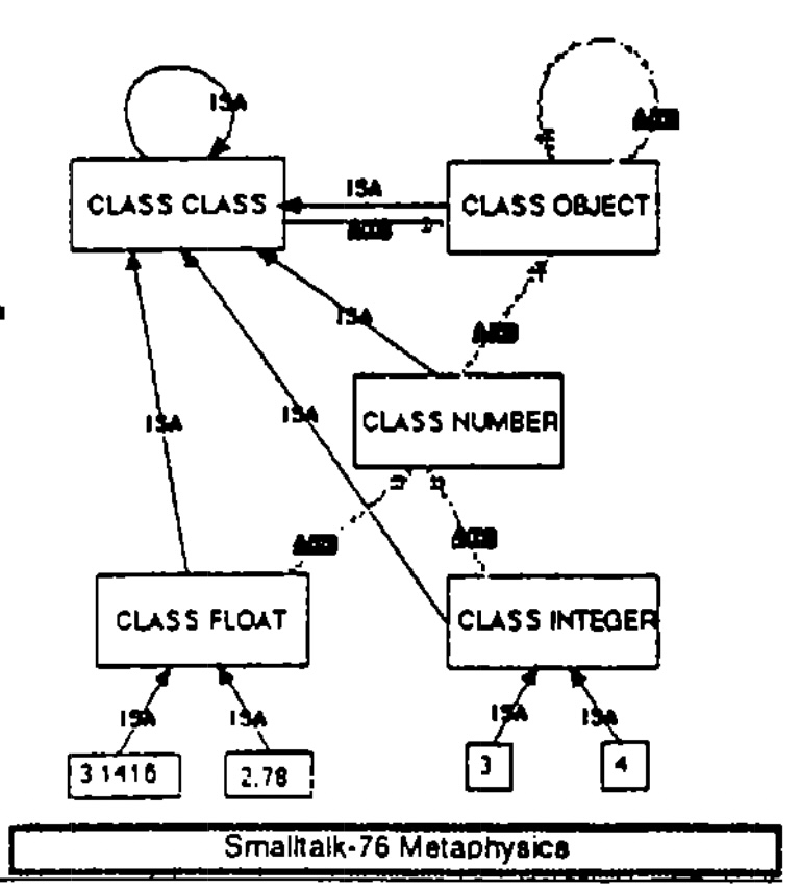
\includegraphics[width=0.8\textwidth]{pictures/smalltalk-76-metaphysics.pdf}
\end{center}
\caption{Smalltalk-76 Metaphyics. From ``\textit{The Early History of
    Smalltalk}'' \cite{kay-history-smalltalk-hopl1993}''. Reproduced
  with permission.}
\label{st-76-metaphysics}
\end{figure}


\subsection{Interpretation} 

The point of these laws, structures, and metaphysics is to execute
Smalltalk programs. Following on from Simula, Smalltalk embodies the idea of
``programming as simulation'': 

\begin{quotation}
\textit{A program execution is regarded as a physical model,
  simulating the behaviour of either a real or an imaginary part of
  the world.}
\end{quotation}
\begin{flushright}
Object-Oriented Programming in BETA \cite{beta}.
\end{flushright}

\noindent For this article, the most important facet of this statement
is the insistence of computation as ``physical model'', a process that
will be embodied via electronic or quantum devices on actual
hardware. (This is in contrast to rather more zipless models of
programming and computation in functional, logical, or quantum
orientation).  For Smalltalk systems, execution is modelled by
exchanges of messages between objects, which is to say a Smalltalk
program.  Traditionally these are modelled as bytecode interpreters:
the methods stored by class objects are arrays of bytes, and the
system implements the methods by interpreting those bytes. (Ingall's
and Kay's HOPL papers give much more details on the evolution of this
design).  The bytecode interpreter is stack based, rather like a
FORTH: arguments are pushed onto a stack: method execution pops its
arguments off the stack and pushes its return value back on.

Figure~\ref{st-76-step} shows the core of the Smalltalk code which
comprises the specification of the Smalltalk-76 bytecodes. This method
reads a byte from the currently execution method, then splits it into
two four-bit ``syllables''. The first syllable, the high bits
(``\textsf{byte|16}'') is used determines the general type of the byte
code -- indeed for many bytecode it determines the entirity of the
operation. The second syllable (``\textsl{lobits}'') can either
identify a particular operation (as in the store, pop, and return
operations in bytecode group~11), or supply a 4-bit operand for an
operation specfied by the first syllable.  See e.g.\ group~6 which
pushes commonly used constants onto the stack, or groups 1--5 which
push values from different types of variables onto the stack.
Groups~9-11 are often called ``extended bytecodes'' because they
provide operations with operands that cannot fit into a 4-bit
syllable, implemented by calling ``\textsf{self nextbyte}'' which
retrieves the nexts byte from the stream.

\begin{figure}[htb]
\begin{center}
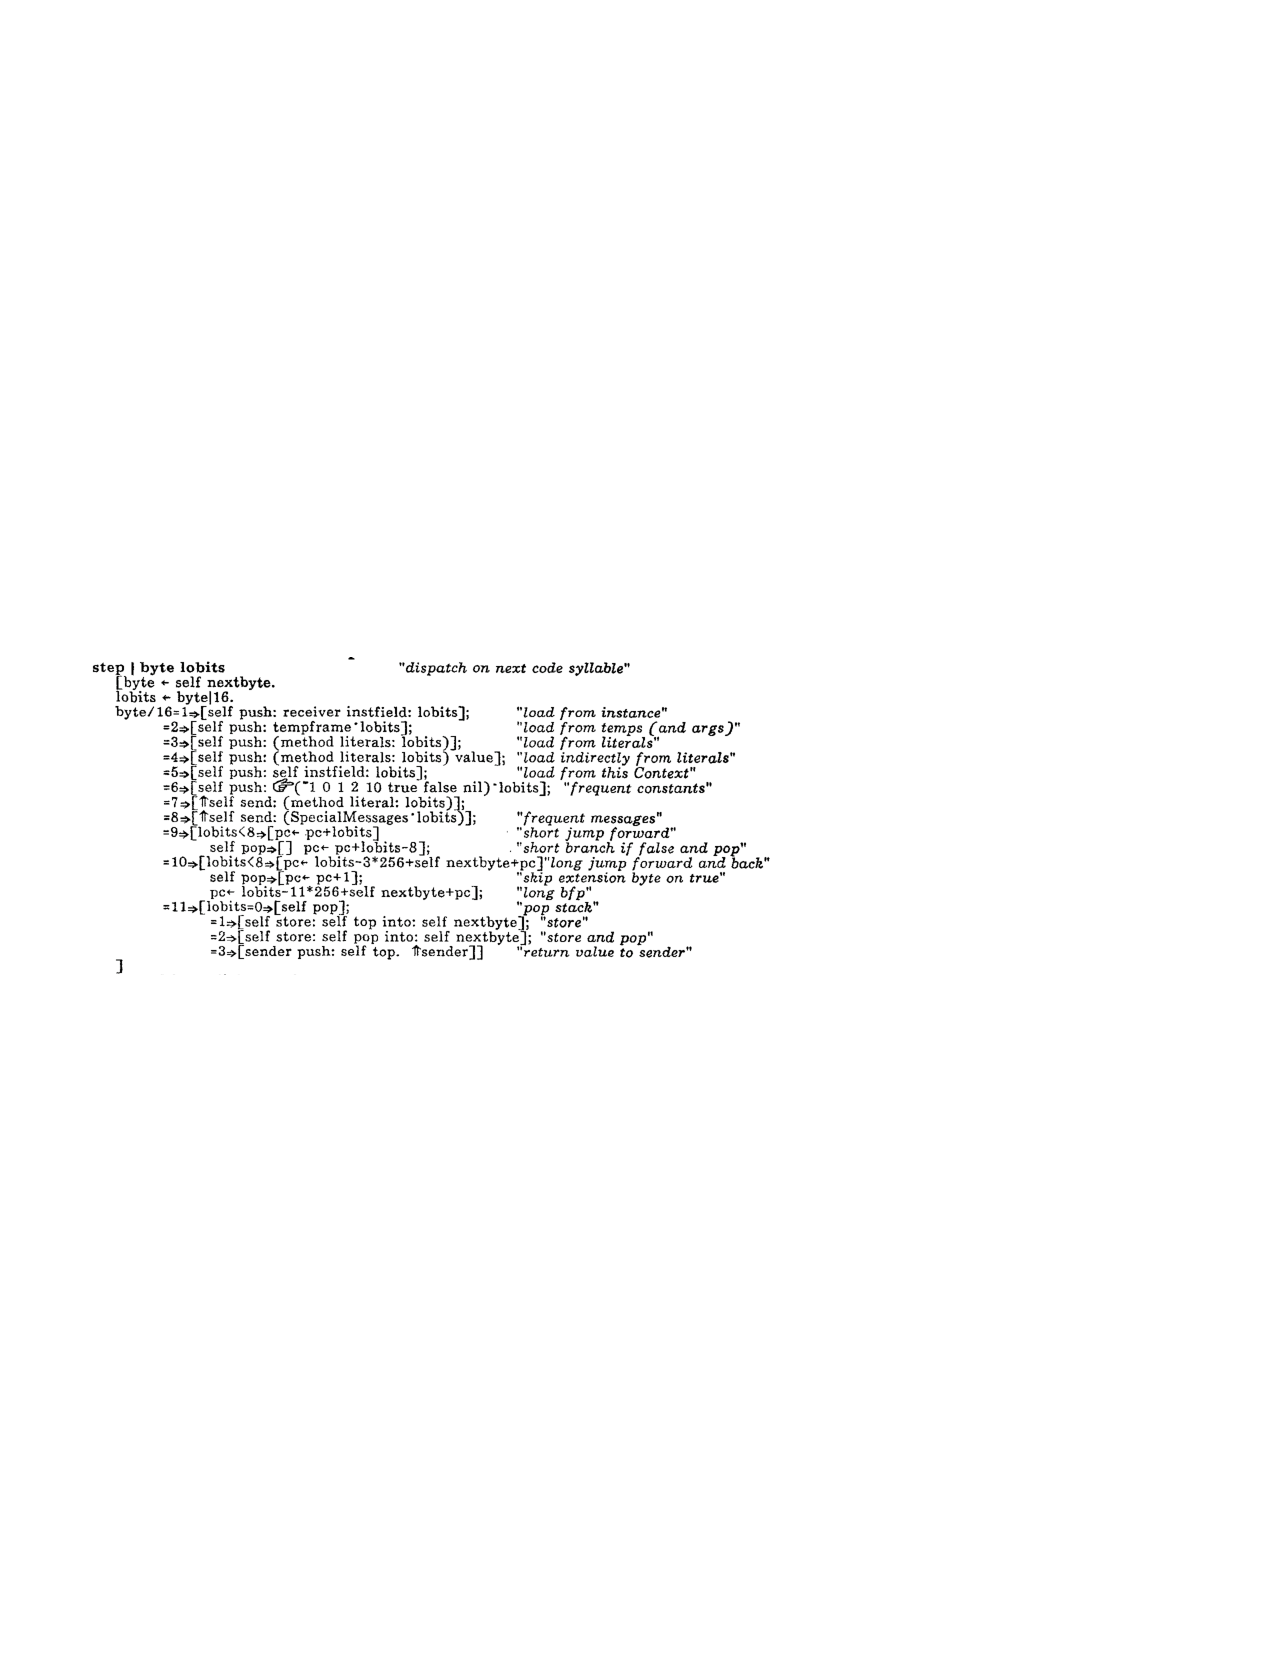
\includegraphics[width=1.0\textwidth]{pictures/st76-step.pdf}
\end{center}
\caption{Smalltalk-76 bytecode decode loop. From ``\textit{The
    Smalltalk-76 Progrmaming System Design and Implementation}''
  \cite{ingalls-smalltalk76-popl1978}''. Reproduced  
  with permission.}
\label{st-76-step}
\end{figure}

Figure~\ref{st-76-store} shows how the store bytecodes are handled,
via a separate ``\textsf{store: val into: field}'' method
Note how the invocation of ``\textsf{store: val into: field}'' in
group~11 in figure~\ref{st-76-step} uses \textsf{nextbyte} to get an
8-bit index of potential store locations.


\begin{figure}[htb]
\begin{center}
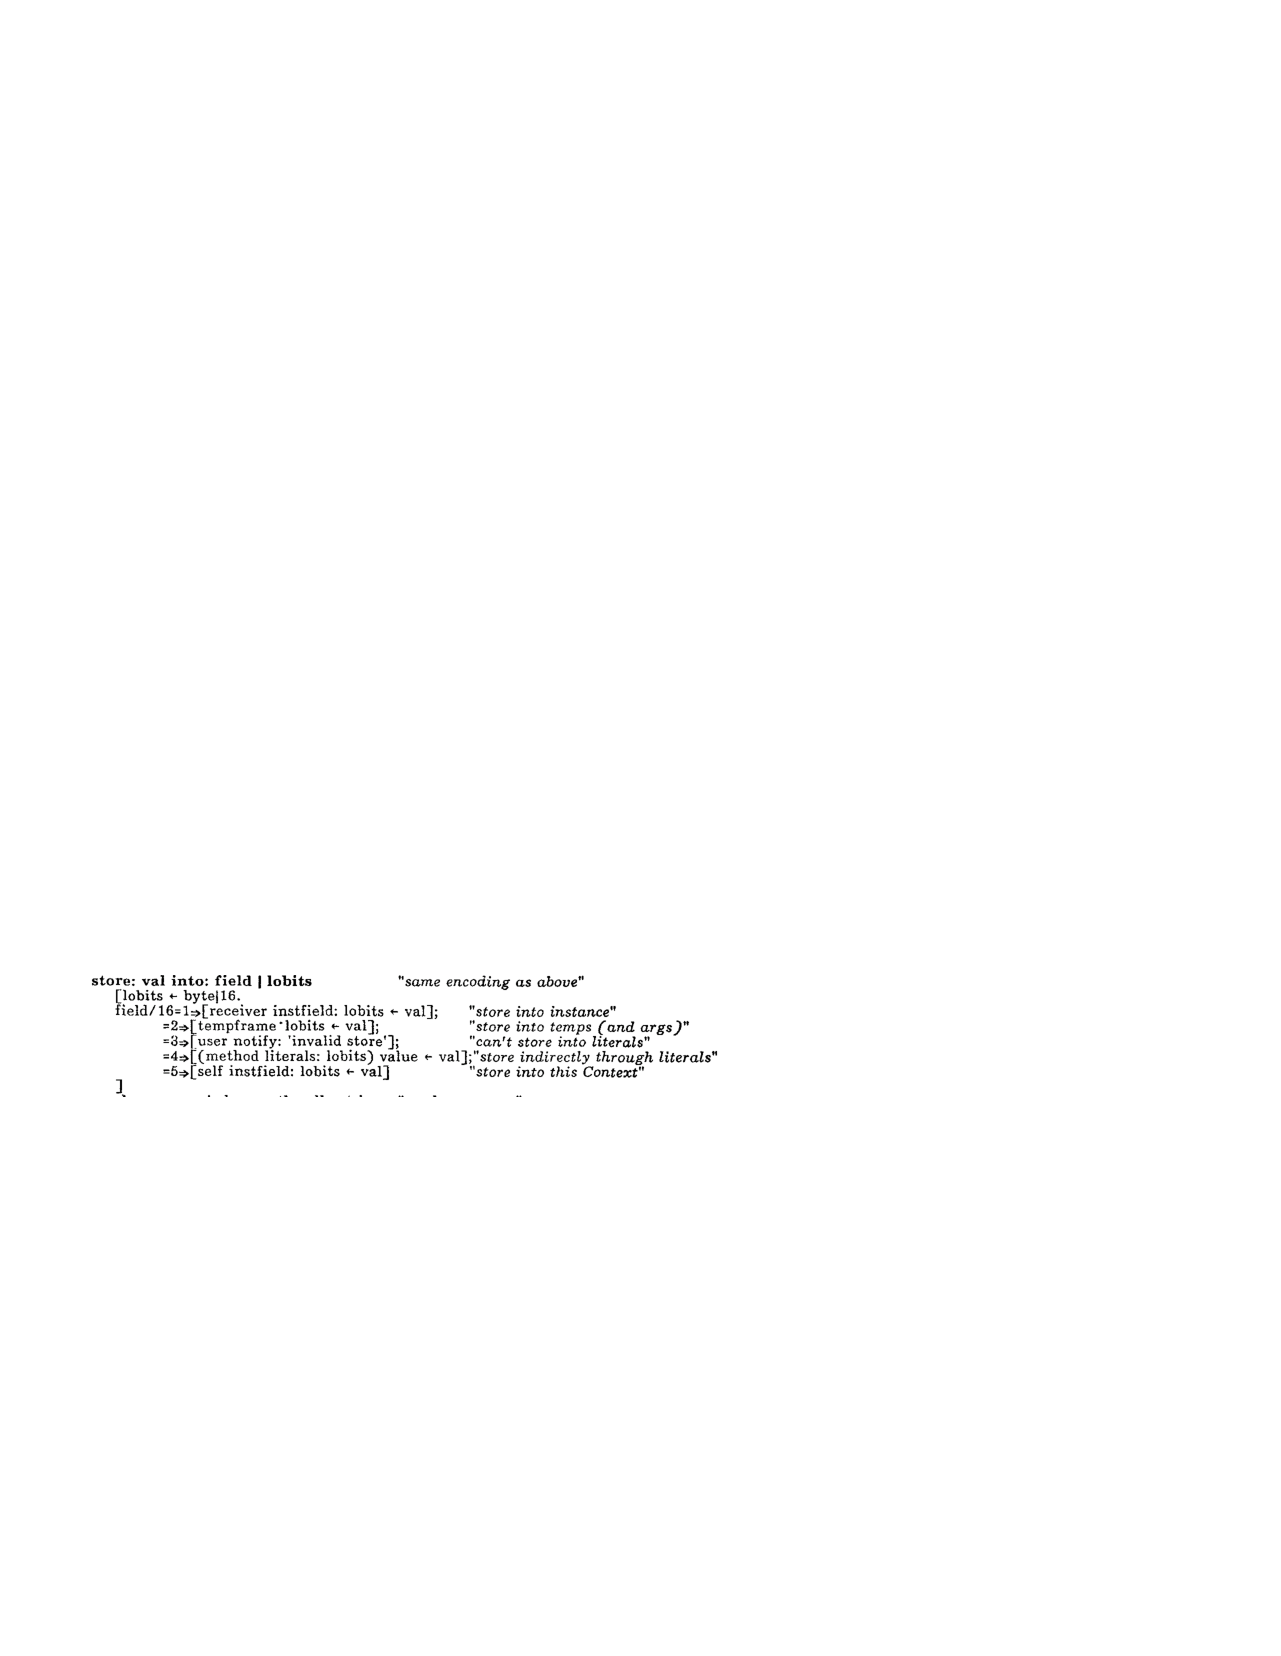
\includegraphics[width=1.0\textwidth]{pictures/st76-store.pdf}
\end{center}
\caption{Smalltalk-76 store bytecode implementation. From ``\textit{The
    Smalltalk-76 Progrmaming System Design and Implementation}''
  \cite{ingalls-smalltalk76-popl1978}''. Reproduced  
  with permission.}
\label{st-76-store}
\end{figure}

Finally figure~\ref{st-76-send} shows the implementation of ``message
sending'' (aka ``dynamic dispatch'' or ``method invocation'' or
``apply'') in Smalltalk-76.  The ``\textsf{send: message}'' method
will be called with an object naming the messagte that has been sent,
i.e.\ the method to be called. The second and fouth line then
implement each stage of the ``\verb+=> ->*+'' rule (one step along the
instance-of relationship, then steps as necessary up the inheritance
relationship). This is called with (a reference to) the reciever
object on the top of the stack. the first line of the method body gets
the top of the stack (``\textsf{self top}'') and then traverses one
step along the instance-of relationship by calling
{``\textsf{class}''} to get that object's class, which will then be
placed into the ``\textsf{class}'' local variable of the
interpreter's method. The class object is then asked to
``\textsf{lookup:}'' the (``\textsf{message}'') in its method
dictionary, and loops over the lookup until the method is found or the
interpreter runs off the top of class ``\textsf{Object}''.   This
lookup involves walking up the inheritance hierarchy from a class to
its superclass --- the code  ``\textsf{class <- class superclass}''
first traverses up from the current ``\textsf{class}'' that has just
been searched to its ``\textsf{superclass}'', and then stores that
superclass into the interpreter's ``\textsf{class}'' local variable.

\begin{figure}[htb]
\begin{center}
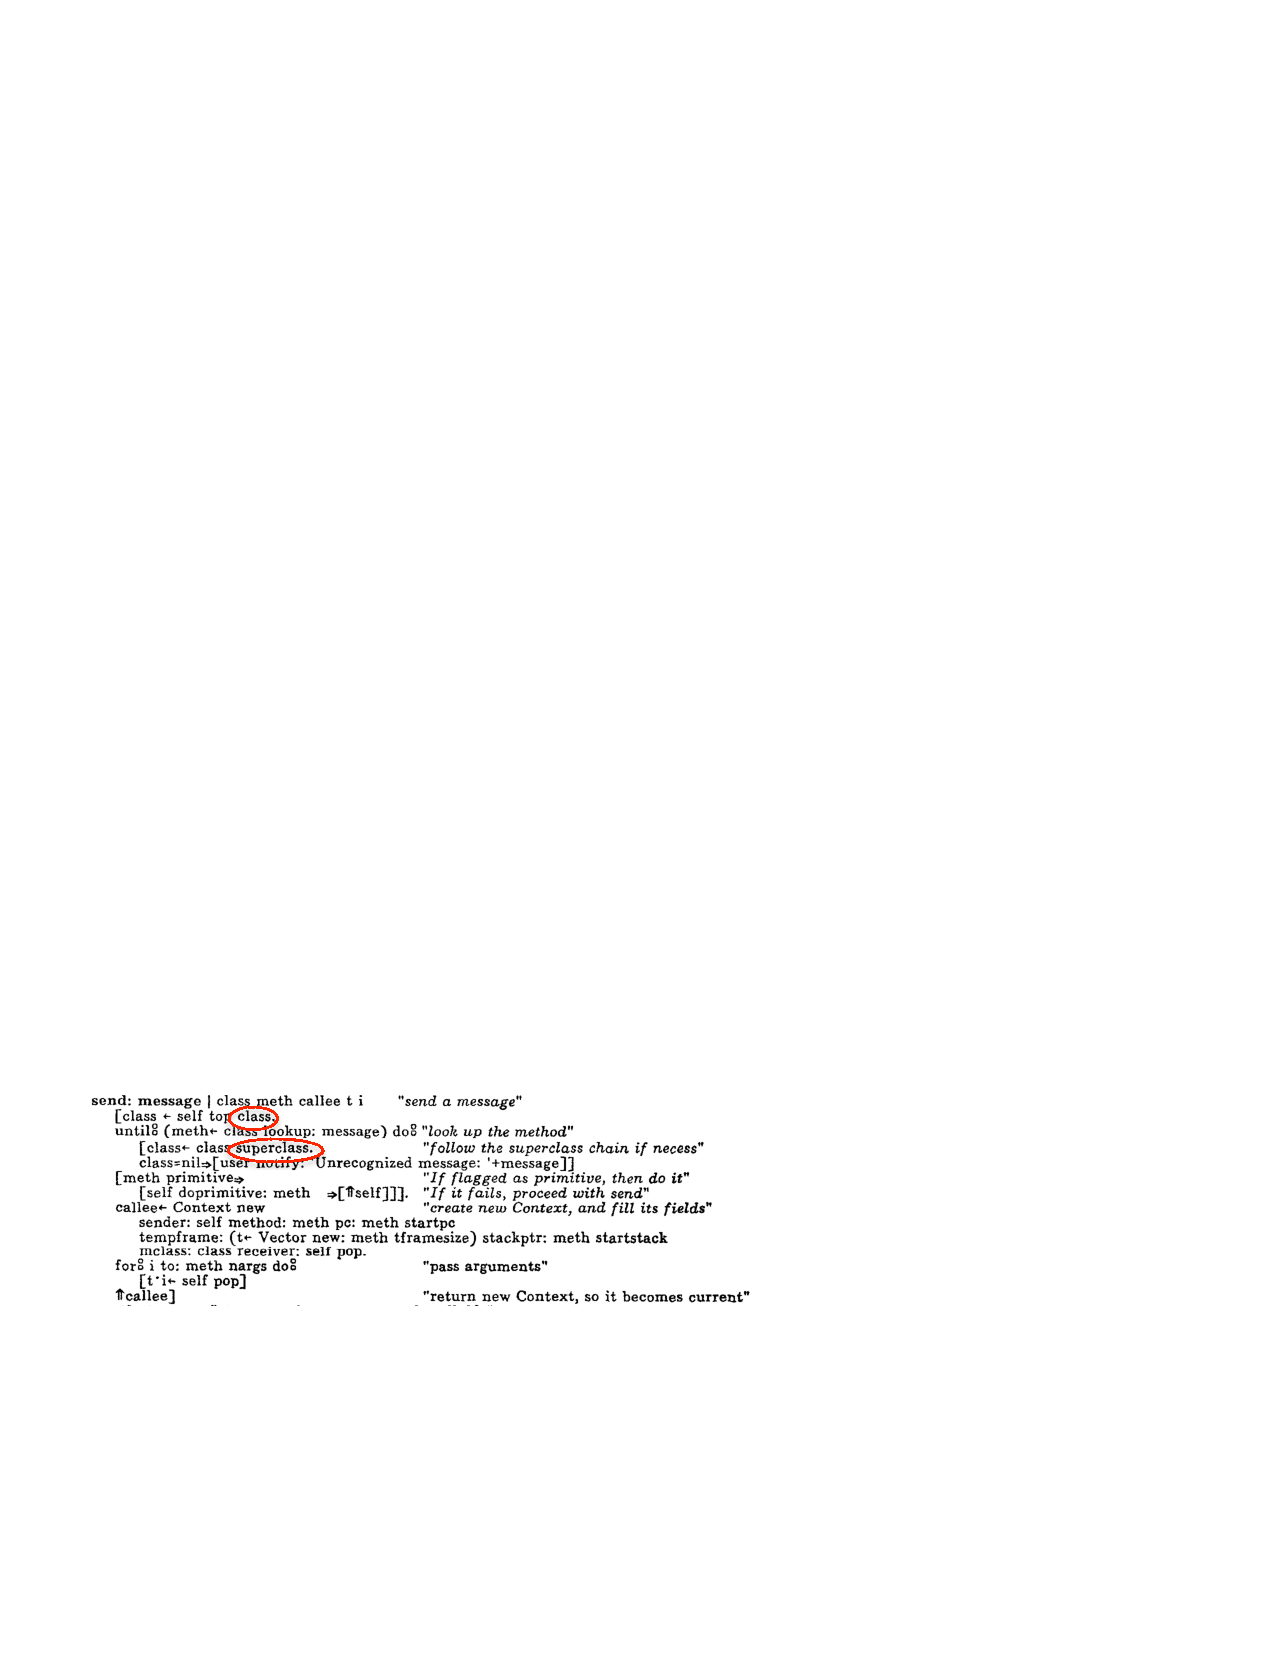
\includegraphics[width=1.0\textwidth]{pictures/st76-send.pdf}
\end{center}
\caption{Smalltalk-76 send bytecode implementation. From ``\textit{The
    Smalltalk-76 Progrmaming System Design and Implementation}''
  \cite{ingalls-smalltalk76-popl1978}''. Reproduced with permission.}
\label{st-76-send}
\end{figure}


\section{Smalltalk-80}


and Sequeak and Pharo and and and



metaclasses - problem (init / construcors(); 
solutoin metacalsses;
running metaclassses on ST76






bytecodes go over in detail





\section{Ruby}

ruby metamodel.



does ruby have byteodes.
arpparenly yes.

\url{https://en.wikipedia.org/wiki/YARV}

so sat how iot evolves

has replaced original - \url{https://en.wikipedia.org/wiki/Ruby_MRI}

\section{Python}

Python metamodel




Pytyhonic shite-codes?



extensions - decorators, types, what else?



point I guess is commonalituy of techniques 




\section{Java}

It's Java, Jim, but nmot as we know it.
not as know it Jim!

show how the original metaclass really are soo Smaltlalk076
(and still are I thikn)

perhaps tail ``mirrors'' vs causal reflection?
(forward refe to self secton I guess)



present the byteodes a an evoluton of ST-80 bytecodes
sithj added types to make everything worsd


taolk aouiti self-optimising bytecodes?



briefly fdiscussion subsequent developments: inner classes,
generics, multi-inheirtnace / traits / whatever
as examples of ``abnove the line'' extensions.

  
\section{Lua}


discus Self

discuss ``protoypes'' vs ``classes''

refer back to Ruby eigencalsses,
SMaltlak version cit Foote'n'Noble ECOOP way back when./

talk about maps - so classes are ``below the line''

talk about ``post-Smalltalk'' super-minimal bytecode set.

draw a long bow and make the argument it's close enough\ldots
  
\section{Lua}



discus Lua.

talk about beautiful C code.

argument shouldn't be that hard...

draw a long bow and make the argument it's close enough\ldots
  
\section{Javascript}


discuss JS.

draw a long bow and make the argument it's close enough\ldots
  
\section{Conclusion}

If Smalltalk did not exist, it would be necessary to reinvent it


Smaltlalks design and technologicla determinism.

Smtallk (butecodewd) vs lisp (S-expressions).

  

\acks
This work is supported in part by the Royal Society of New Zealand Te
Ap\={a}rangi  Marsden Fund Te P\={u}tea Rangahau a Marsden grants
VUWU1815 and CRP2101, an Amazon Research Award, and an INRIA
International Visiting Chair.


\end{document}






  
st76
class decs / object strucutre & inheritance
(prefixing?)

object struvute - message sending and inheritance 
tagged integers 
arrays

examples:

ST80 as ST7- example
**ST80 metamodel
  

Ruby
eigneclasses = foote and co
type inferenve


python
(mention ABC?)
storage strageies
what else in ST?




traits in JAVA 
MI in Smtalltalk

TYPED BYTECODES java
TRAINS - in smaltalk - in JAVA



SElfmaps are classes 


iLua???
